\chapter{Lab 2 - Processes}

Congratulations on completing the first lab! Hopefully you have had a chance to play
around with the MOS kernel and have a better understanding of its structure.

In this lab, we will be looking at the process management in MOS.

\section{Files in MOS that relate to process management}

\begin{figure}[ht]
    \centering
    \raisebox{-.5\height}{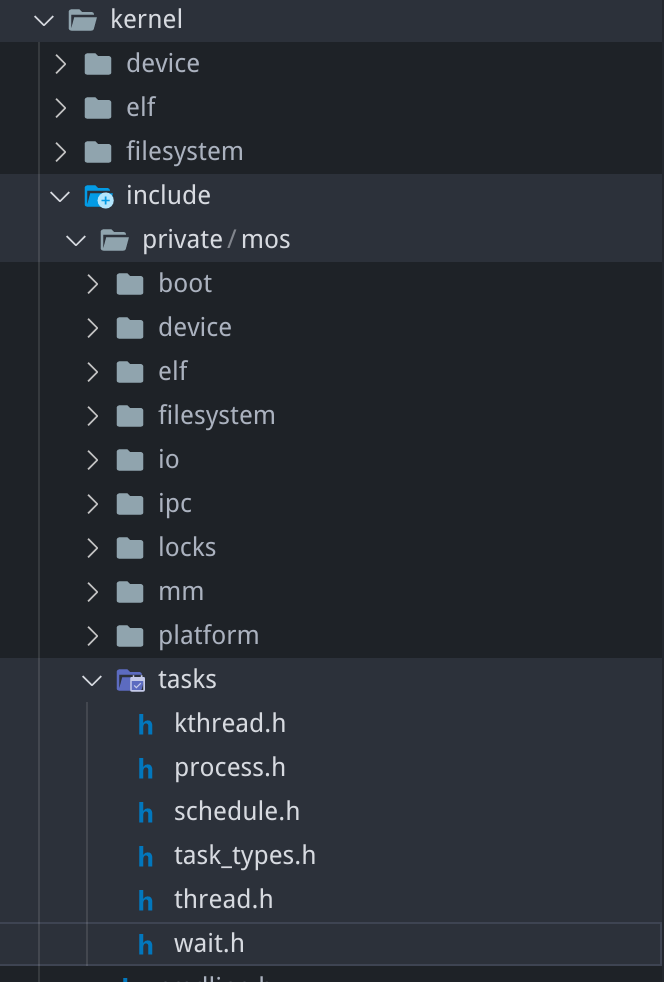
\includegraphics[width=0.4\textwidth]{assets/c2.headers.png}}
    \raisebox{-.5\height}{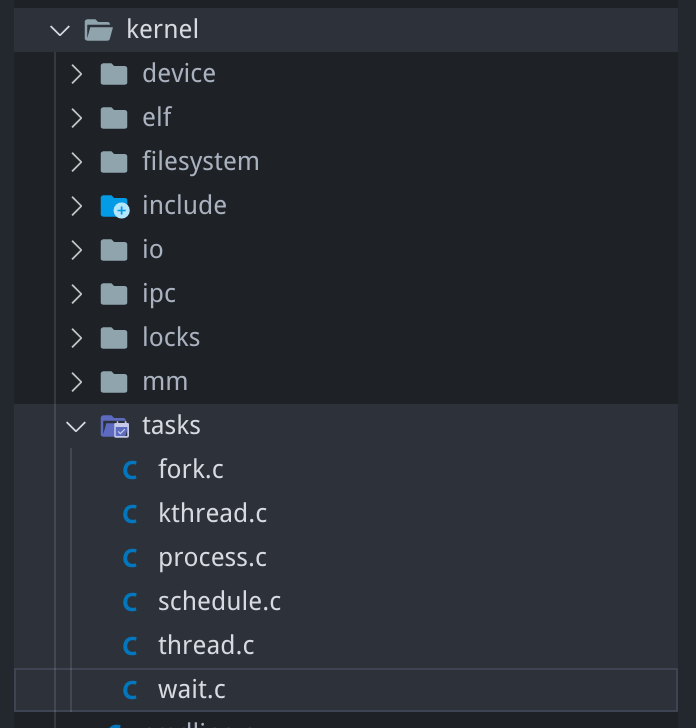
\includegraphics[width=0.4\textwidth]{assets/c2.sources.png}}
    \caption{The header and source files in \texttt{kernel/tasks}}
    \label{fig:mos-process-management-files}
\end{figure}

The process management in MOS is implemented in the \texttt{kernel/tasks} directory, and the
corresponding header files are in \texttt{kernel/include/private/mos/tasks} as shown in
Figure \ref{fig:mos-process-management-files}.

\begin{note}
    \item The \texttt{kernel/include/private} directory is a convension used in MOS, which
    contains the header files that are \textbf{not} meant to be used by userspace programs.
\end{note}

\section{Process Control Blocks}

You have learnt about this in the lecture: `a process is a program in execution', and a process
control block (PCB) is a data structure that contains information about a process.

Now, let's look at the PCB structure in MOS. The PCB is defined as a struct named \texttt{process\_t}
in \texttt{task\_types.h}.

Several fields are defined in PCB, but we will only look at the ones that are relevant to
process management, which are:

\begin{itemize}
    \item \texttt{pid}: The process id.

          Each process has a unique id, this is what MOS uses to identify a process.\\
          In MOS, the process id is an unsigned 32-bit integer, and this number always
          increases.

    \item \texttt{name}: The name of the process, nothing interesting here.

    \item \texttt{parent}: The parent of the process, this is a pointer to the PCB of the parent.

          Unlike most animals, a process can only have one parent. The \texttt{init}
          process lives at the root of the process tree, it's fun to think about it being its own
          parent.

    \item \texttt{files}: A list of opened files.

          This is a staticly allocated array of size \texttt{MOS\_PROCESS\_MAX\_OPEN\_FILES},
          the value of which is determined by the kernel configuration.

          Each time a file is opened, an \texttt{io\_t} that represents an IO object (file, pipe, etc.)
          is added to this array, and the index of such an object is returned to the user program.

          This index is called a `file descriptor', or `fd' for short. The user program can use
          this number to refer to the file in the future.

          The \texttt{io\_t} structure is defined in \texttt{kernel/include/private/mos/io/io.h},
          the details of which is probably beyond the scope of this lab.

    \item \texttt{threads}: A list of threads.

          To be honest, this list is unnecessary, because we already have a thread table elsewhere
          in MOS, the list here is just a convenience for the kernel to iterate over all threads
          of a specific process, (think about it as a cache).

    \item \texttt{pagetable}, \texttt{mmaps}: The page table and a list of mapped memory regions,
          these two will be discussed in later chapters.
\end{itemize}

\section{Thread Control Blocks}

You may have noticed that the PCB above is \textit{little bit} different from the one in the
lecture: It has neither `process state' nor `stack/heap/text memory regions'.

Because, in MOS, a thread is basic unit of execution instead of a process. Thus it's the thread that has a
`state' and a `stack', and the process is just a collection of threads.

The thread control block is defined in the same file as the PCB. You can see that it contains
a \texttt{tid} for a thread id, and a \texttt{state} field to indicate the state of the thread,
its owner process, two stacks for the kernel and user mode respectively.

There's also a \texttt{context} pointer, this will be used in context switching, we'll look at
that later.

\section{Process Creation}

A process has to be created from a `program' (a binary executable file) in order to be
executed. WLOG, creating a process involves the following steps:

\begin{enumerate}
    \item Load the program into the memory.
    \item Create a PCB and populate the fields.
          \begin{enumerate}
              \item Allocate and initialize the PCB.
              \item Allocate a user-mode page table.
              \item Parse the program and map corresponding memory regions into the page table.
              \item Allocate a heap for the process in the user-mode page table.
                    (part 2 in Figure \ref{fig:mos-process-memory-layout})
              \item Add the PCB to the process table.
          \end{enumerate}
    \item Create a main thread.
          \begin{enumerate}
              \item Allocate and initialize the TCB for the main thread.
              \item Allocate \textbf{both} the user-space and kernel-space stack space for the thread.
                    (part 2 in Figure \ref{fig:mos-process-memory-layout})
              \item Add the thread to the thread table.
              \item Set thread state to \texttt{CREATED}.
          \end{enumerate}
    \item (optionally) schedule to the new thread.
\end{enumerate}

The figure \ref{fig:mos-process-memory-layout} shows the memory layout of a process in MOS
after its creation.

\begin{figure}
    \definecolor{lightcyan}{rgb}{0.8,1,1}
    \definecolor{lightgreen}{rgb}{0.56,0.93,0.56}
    \definecolor{lightlightgreen}{rgb}{0.8,1,0.8}
    \definecolor{gray}{rgb}{0.7,0.7,0.7}
    \definecolor{lightred}{rgb}{1,0.7,0.71}

    % \memsection{end address}{start address}{height in lines}{text in box}{color}
    \newcommand{\memsection}[6][lrtb]{%
        \bytefieldsetup{bitheight=#4\baselineskip}%
        \bitbox[]{10}{
            \texttt{#2} \\ % end addressd
            \vspace{#4\baselineskip}
            \vspace{-2\baselineskip}
            \vspace{-#4pt}
            \texttt{#3} % start address
        }
        \bitbox[#1]{16}[bgcolor=#5]{\small #6}
    }

    \newcommand{\memgap}[2][lrtb]{
        \bytefieldsetup{bitheight=#2\baselineskip}
        \bitbox[#1]{16}[bgcolor=gray]{\small Gap}
    }

    Color Description:
    \colorbox{gray}{\textbf{Unavailable}}
    \colorbox{lightred}{\textbf{Kernel Only}}
    \colorbox{lightgreen}{\textbf{User Read-Only}}
    \colorbox{cyan}{\textbf{User Read-Write}}

    \begin{center}
        \begin{bytefield}{24}
            \memsection{0xffffffff}{0xC0000000}{6}{lightred}{Kernel}\\
            \memgap{6}\\
            \begin{leftwordgroup}{2. Address determined\\ by the MOS Kernel}
                \begin{rightwordgroup}{4. Per-thread\\Memory Regions}
                    \memsection{\dots}{}{2}{lightred}{\scriptsize{Kernel-Mode Thread Stacks \dots}}\\
                    \memsection{}{}{2}{cyan}{\scriptsize{User-Mode Thread Stacks \dots}}
                \end{rightwordgroup}\\
                \begin{rightwordgroup}{4. \textbf{Main} Thread\\Memory Regions}
                    \memsection{}{}{2}{lightred}{\scriptsize{Kernel-Mode \textbf{Main} Thread Stack}}\\
                    \memsection{0x60020000}{\dots}{2}{cyan}{\scriptsize{User-Mode \textbf{Main} Thread Stack}}
                \end{rightwordgroup}\\
                \memgap{2}\\
                \begin{rightwordgroup}{3. Per-process\\Memory Regions}
                    \memsection[ltr]{}{}{5}{lightcyan}{\textit{Future} Heap \textit{Area}}\\
                    \memsection[lbr]{}{0x40000000}{3}{cyan}{\texttt{\large{$\uparrow$}} \\ Heap}
                \end{rightwordgroup}
            \end{leftwordgroup}\\
            \memgap{4}\\
            \begin{leftwordgroup}{1. Address determined\\ by the Program Header}
                \memsection{\dots}{}{3}{cyan}{\texttt{.bss} Section}\\
                \memsection{}{}{3}{cyan}{\texttt{.data} Section}\\
                \memsection{}{}{2}{lightgreen}{\texttt{.rodata} Section}\\
                \memsection{}{0x08048000}{2}{lightgreen}{\texttt{.text} Section}
            \end{leftwordgroup}\\
            \memsection{}{0x00000000}{5}{gray}{Unavailable}\\
        \end{bytefield}
    \end{center}
    \caption{The memory layout of a process in MOS (Not to scale)}
    \label{fig:mos-process-memory-layout}
\end{figure}

\textbf{\textit{TODO: Add exercises}}

\section{The famous \texttt{fork()} system call}

You may have known that the \texttt{fork()} system call is used to create a new process, which seems
to be the same as what we have just discussed. However, think about the following question:

\begin{quote}
    What if we want to create a new process that is exactly the same as the current process, instead
    of creating a new process from a program?
\end{quote}

\dots
